\documentclass[10pt]{article}
\usepackage[polish]{babel}
\usepackage[utf8]{inputenc}
\usepackage[T1]{fontenc}
\usepackage{amsmath}
\usepackage{amsfonts}
\usepackage{amssymb}
\usepackage[version=4]{mhchem}
\usepackage{stmaryrd}
\usepackage{graphicx}
\usepackage[export]{adjustbox}
\graphicspath{ {./images/} }

\title{KLASY PIERWSZE I DRUGIE }

\author{}
\date{}


\begin{document}
\maketitle
\begin{enumerate}
  \item Na każdym polu szachownicy \(11 \times 11\) siedzi konik polny. W pewnym momencie koniki przeskakują ze swojego pola na pole sąsiednie (tzn. pole o wspólnym boku). Rozstrzygnij, czy jest możliwe, aby po tym ruchu wszystkie pola nadal były zajęte. Odpowiedź uzasadnij.
  \item W turnieju tenisa stołowego wzięło udział 50 zawodników. Każdy zawodnik rozegrał jeden mecz z każdym innym zawodnikiem, nie było remisów. Czy możliwe jest, aby każdy z uczestników wygrał tę samą liczbę meczów? Odpowiedź uzasadnij.
  \item Punkty \(K\) i \(L\) leżą na bokach \(A D\) i \(B C\) równoległoboku \(A B C D\), przy czym \(A K=L C\). Punkt \(P\) leży na boku \(C D\). Pokazać, że jeśli prosta \(K L\) przecina proste \(A P\) i \(B P\) odpowiednio w punktach \(M\) i \(N\), to pole trójkąta \(P M N\) jest równe sumie pól trójkątów \(A K M\) i \(B L N\).\\
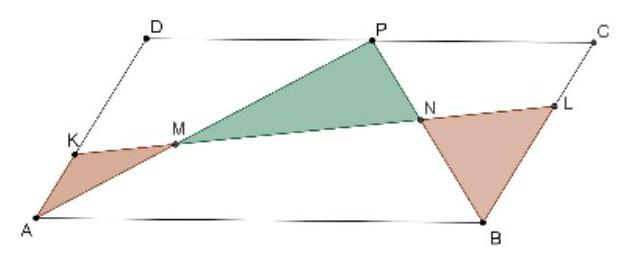
\includegraphics[max width=\textwidth, center]{2024_11_21_b72d51b763316a99ebb1g-1}
\end{enumerate}

\section*{KLASY TRZECIE}
\begin{enumerate}
  \item Dane są punkty \(A, B, C, D\) leżące w tej kolejności na okręgu. Niech \(S\) będzie środkiem łuku AB, U środkiem łuku BC, T środkiem łuku CD i V środkiem łuku DA tego okręgu. Udowodnij, że odcinki ST i UV są prostopadłe.
  \item Czworokąt wypukły podzielono przekątnymi na cztery trójkąty. Pola \(S_{1}, S_{2}, S_{3}, S_{4}\) tych trójkątów są liczbami całkowitymi. Udowodnij, że liczba \(S_{1}+S_{2}+S_{3}+S_{4}\) jest złożona.
  \item Udowodnij, że istnieje nieskończenie wiele par liczb naturalnych \((a, b)\), dla których liczba \(4^{a}+4^{b}+4^{a+b}\) jest kwadratem liczby całkowitej.
\end{enumerate}

\end{document}